\documentclass{beamer}

\usepackage[utf8]{inputenc}
\usepackage{ctex}

\usepackage{graphicx}
\usepackage{subcaption}

\usepackage{amsmath}
\usepackage{algorithm}
\usepackage{algpseudocode}



\graphicspath{ {images/} }

\usetheme{Madrid}
%\usetheme{Antibes}


\title[侦测隐藏敌人状态]{使用贝叶斯方法探测隐藏敌人状态 }
\author{卓越羿}
\institute[SICNU]{四川师范大学数学与软件科学学院}
\date{2018}

\begin{document}

\frame{\titlepage}

\begin{frame}

\frametitle{战斗的概率模型}

给定友军和敌军,战斗被期望在它们“之间”发生,如何建模?

利用一个朴素贝叶斯分类器的“难以分类水平”定义“冲突水平”,再结合一个距离因子。

$$
P(x,y) \propto sigm(t (P_\text{ally}(x,y) (1-P_\text{ally}(x,y)) - \theta_0)) sigm(t(-\min_{u} distance + \theta_1))
$$

$$
P_\text{ally}(x,y) = \frac{
N(x\mid \mu^A_X ,\sigma^A_X) N(y \mid \mu^A_Y, \sigma^A_Y)
}{
N(x \mid \mu^A_X , \sigma^A_X) N(y \mid \mu^A_Y , \sigma^A_Y) + 
N(x \mid \mu^E_X , \sigma^E_X) N(y \mid \mu^E_Y , \sigma^E_Y)
}
$$


\end{frame}

\begin{frame}
\frametitle{葛底斯堡战役}

\begin{figure}[htb]
  \begin{subfigure}[b]{0.26\linewidth}
    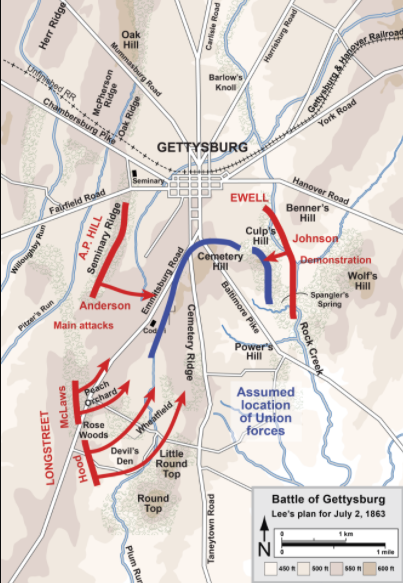
\includegraphics[width=\linewidth]{gettysburg-map.png}
    \caption{葛底斯堡战役第二天的战场示意图}
  \end{subfigure}
  \begin{subfigure}[b]{0.26\linewidth}
    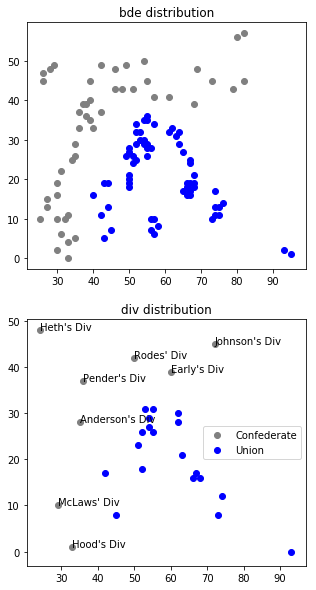
\includegraphics[width=\linewidth]{gettysburg-model.png}
    \caption{旅/师级单位位置坐标}
  \end{subfigure}
  \label{fig:gettysburg}
\end{figure}

\end{frame}

\begin{frame}

\frametitle{模型在葛底斯堡数据上的效果}

\begin{figure}[htb]
  \centering
  \begin{subfigure}[b]{0.49\linewidth}
    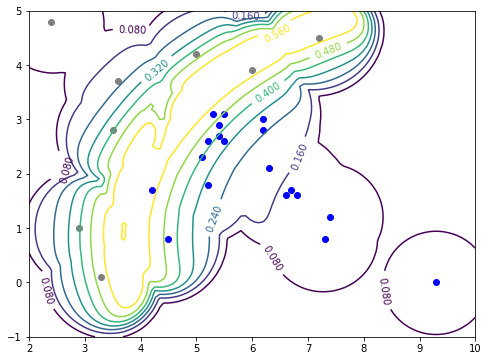
\includegraphics[width=\linewidth]{gettysburg-forward.png}
    \caption{未标准化的战役发生概率}
  \end{subfigure}
  \begin{subfigure}[b]{0.49\linewidth}
    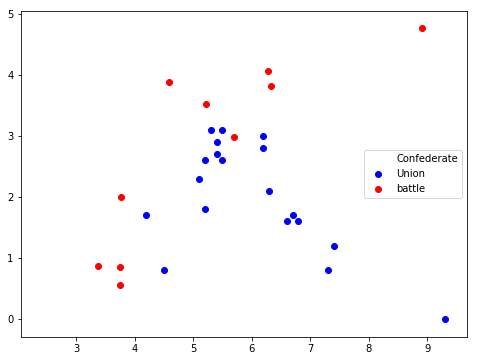
\includegraphics[width=\linewidth]{gettysburg-sample.png}
    \caption{一次采样结果+友军位置构成的模型所用数据}
  \end{subfigure}
  \caption{正向生成模型与一次采样结果}
  \label{fig:gettysburgTwo}
\end{figure}

\end{frame}

\begin{frame}

\frametitle{主要使用方法:变分推断}

利用正态分布族近似精确后验分布,近似优劣以降低KL散度为准:

$$
KL(q||p) = E_q \left( \log \frac{q(\theta \mid \mu,\omega)}{p(\theta \mid x)} \right)
$$

$p(\theta \mid x)$无法计算,转而等价地最大化置信下界$ELBO$

$$
\mathrm{ELBO} = E_q (\log p(x,\theta)) - E_q(\log q(\theta)) 
$$

$E_q(\cdot)$可用蒙特卡洛积分近似计算

\end{frame}

\begin{frame}
\frametitle{变分推断算法:自动微分变分推断(ADVI)}

\begin{algorithm}[H]

\tiny

\caption{自动微分变分推断(平均场,不考虑变换)}
\begin{algorithmic}[1]
\Procedure{ADVI}{$\mathbf{\mu},\mathbf{\omega},lr,M,step$}  \Comment{$\mathbf{\mu},\mathbf{\omega}$ 是初始值,$M$是随机积分采样个数}
    \For{$s$ in $1:step$}
        \State $\hat{\nabla}_\mathbf{\mu} \gets \mathbf{0}$
        \State $\hat{\nabla}_\mathbf{\omega} \gets \mathbf{0}$
        \For{$i$ in $1:M$} 
            \State $\mathbf{\eta} \sim N(\mathbf{0},\mathbf{I}) $ \Comment{从多元标准正态分布中采样,下同}
            \State $\hat{\theta} \gets (\mathbf{\eta} * \exp(\mathbf{\omega})) + \mathbf{\mu}$ \Comment{$*$即按元素对应相乘}
            \State $\hat{\nabla}_\mathbf{\mu} \gets \hat{\nabla}_\mathbf{\mu} + (\nabla_\theta \log p(x,\theta)|_{\hat{\theta}})$
            \State $\hat{\nabla}_\mathbf{\omega} \gets \hat{\nabla}_\mathbf{\omega} + \hat{\nabla}_\mu * \mathbf{\eta}$
        \EndFor
        \State $\hat{\nabla}_{\mathbf{\mu}} \gets \hat{\nabla}_{\mathbf{\mu}} / M$
        \State $\hat{\nabla}_{\mathbf{\omega}} \gets (\hat{\nabla}_\mathbf{\omega} / M) * \exp(\mathbf{\omega}) + \mathbf{1}$
        \State $\mathbf{\mu} \gets \mathbf{\mu} + lr \hat{\nabla}_{\mathbf{\mu}}$
        \State $\mathbf{\omega} \gets \mathbf{\mu} + lr \hat{\nabla}_{\mathbf{\omega}}$
    \EndFor 
    \State \Return $\mathbf{\mu},\mathbf{\omega}$
\EndProcedure
\end{algorithmic}
\label{alg:advi}
\end{algorithm}

\end{frame}

\begin{frame}
\frametitle{应用:敌对单位位置后验分布估计}

\begin{figure}[htb]
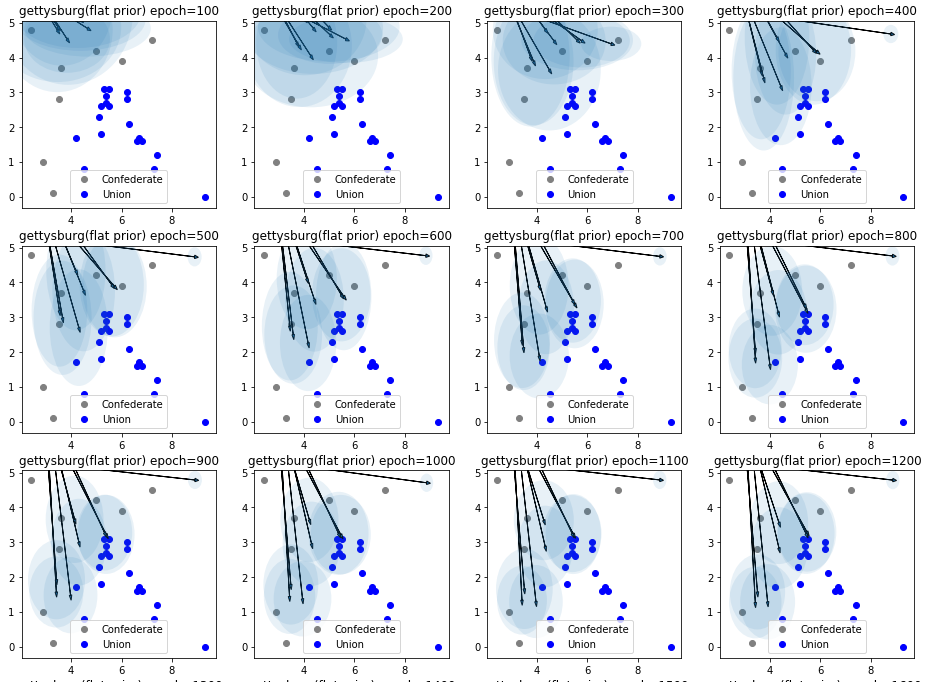
\includegraphics[width=0.8\linewidth]{gettysburg-point-small.png}
\label{fig:gettysburgInit}
\end{figure}



\end{frame}

\begin{frame}
\frametitle{应用:敌对单位存在概率密度估计}

采用正态分布族的变分推断的一大好处就是计算特定敌军单位在特定区域的后验概率十分方便。
从而可以直接计算出任意矩形区域$[x,x+dx]\times[y,y+dy]$中存在任意敌军单位的概率:

\begin{align*}
pe(x,y,dx,dy) = 1-
\prod_i^{N_E}
(1-
& ((\Phi((x + dx - \mu_{X^E_i})/\sigma_{X^E_i}) - \Phi((x - \mu_{X^E_i})/\sigma_{X^E_i})) \\
&  (\Phi((y + dy - \mu_{Y^E_i})/\sigma_{Y^E_i}) - \Phi((y - \mu_{Y^E_i})/\sigma_{Y^E_i})))
)
\end{align*}

%而$\mu_{X^E_i}$是第$i$个敌人的近似后验分布的正态期望参数,另外几个类似。
%这种话就不写在ppt里了,临时解释就是。

从而近似地计算出存在密度:

$$
pe(x,y) = pe(x-\epsilon,y-\epsilon,2\epsilon,2\epsilon)/(4 \epsilon^2)
$$

\end{frame}

\begin{frame}
\frametitle{葛底斯堡战役数据的存在推断收敛过程}

\begin{figure}[htb]
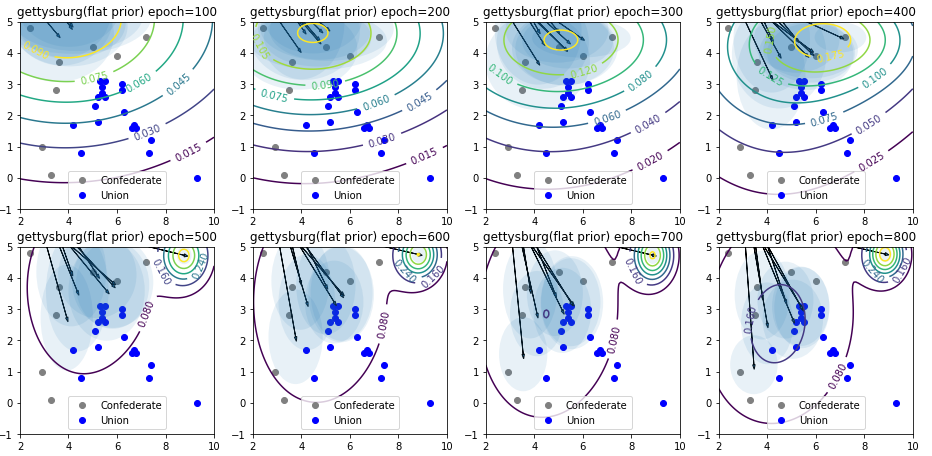
\includegraphics[width=0.99\linewidth]{gettysburg-init-beamer.png}
\label{fig:gettysburgInit}
\end{figure}


\end{frame}

\begin{frame}

\frametitle{其他扩展}

本文也考虑了移动侦测,考虑规模效应的变体。设置不同先验,设置不同初始值,各种数据形态检验模型有效性。
也考虑了比较这个模型以外的几个模型的效果。也讨论了哈密顿蒙特卡洛实现等。具体内容见原文。

\begin{figure}[htb]
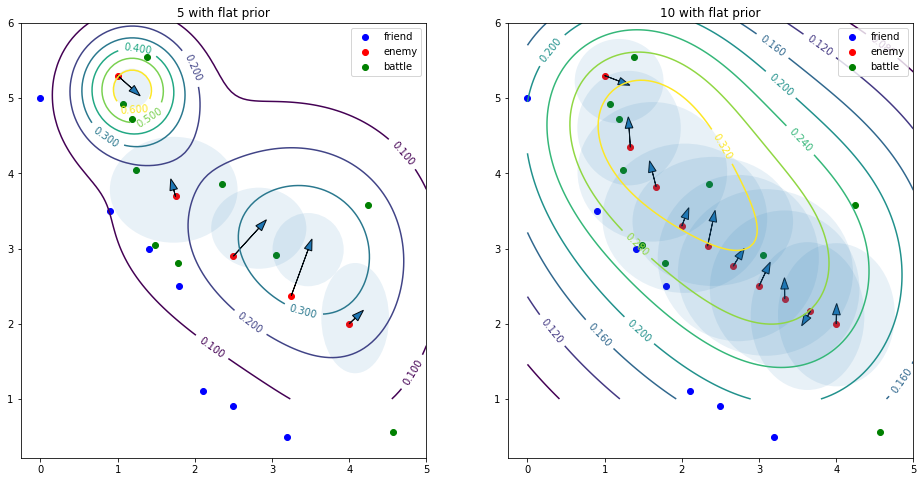
\includegraphics[width=0.7\linewidth]{exist_density.png}
\label{fig:gettysburgInit}
\end{figure}

\end{frame}



\end{document}